\subsection{temperature} 
\begin{figure}[hbt!] 
\begin{subfigure}{0.3\textwidth} 
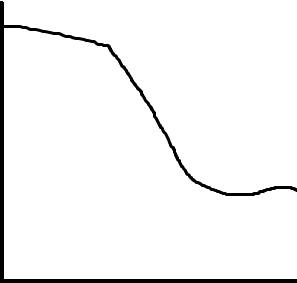
\includegraphics[width=0.9\linewidth]{reports/current_report/images/max_graph_temperature.png}  
\caption{max temperature}  
\end{subfigure} 
\begin{subfigure}{0.3\textwidth} 
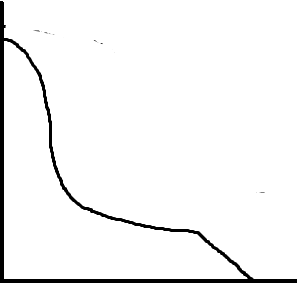
\includegraphics[width=0.9\linewidth]{reports/current_report/images/min_graph_temperature.png}  
\caption{min temperature}  
\end{subfigure} 
\begin{subfigure}{0.3\textwidth} 
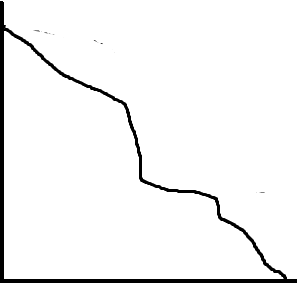
\includegraphics[width=0.9\linewidth]{reports/current_report/images/average_graph_temperature.png}  
\caption{max temperature}  
\end{subfigure} 
\caption{comparison between the minimum and maximum temperature}  
\end{figure} 
\FloatBarrier  
the average temperature during week 1 (5th of December until the 12th of December) was 17 °C.an overview of the temperature images can be seen here:\begin{SCfigure}[0.5][hbt!]
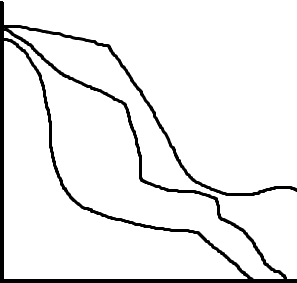
\includegraphics[width=0.6\textwidth]{reports/current_report/images/combined_graph_temperature.png}  
\caption{vectorfield temperature}  
\end{SCfigure} 
\FloatBarrier  
